
\documentclass [12pt, proquest]{uwthesis}[2019]

\usepackage{graphicx}
\usepackage{subfig}
\usepackage{amsmath}
\usepackage{setspace}
\usepackage{lineno}
\usepackage{natbib}

\begin{document}

\title{}
\prelimpages
 
\Title{Development and Deployment of Precision Mechanical Rotation Sensor for Terrestrial Gravitational Wave Observatories}
\Author{M. P. Ross}
\Year{2019}
\Program{Physics}

\Chair{Name of Chairperson}{Title of Chair}{Department of Chair}
\Signature{First committee member}
\Signature{Next committee member}
\Signature{etc}

\copyrightpage

\titlepage  

\setcounter{page}{-1}
\abstract{}

\tableofcontents
\listoffigures

\dedication{\begin{center}To Grace\end{center}}
\textpages
\chapter{Introduction}
\section{Gravitational Wave Theory}
\section{LIGO}
\section{Seismic Isolation}

\chapter{1-m Scale Ground Rotation Sensors}
\section{Tilt Contamination}
\quad At their core seismometers are low frequency spring mass system which measures the difference in motion between the casing and the device's proof mass. Above the resonant frequency of the spring mass system, this allows for accurate measurements of the motion in reference to an inertial frame of any object that the casing is rigidly connected to, be it the ground or a suspended table. Over the past \textbf{some time} this technology has produced devices that are sensitive to \textbf{number and range}. However, these systems are fundamentally susceptible to any stray forces acting on the proof mass.

Of interest here is the contamination due to the rotation of the device within a external gravitational field, namely the field caused by the earth. The rotation in respect to a fixed gravitational force will be referred to as tilt.\footnote{Although a subtle difference, the distinction would be of great consequences if the local gravitational field was varying rapidly. In that case the sensors described here would be of little use as they are rotational sensors not tilt sensors.} From the proof mass's frame, a tilt is equivalent to a rotation of the gravitational force. This yields a horizontal acceleration of the proof mass of:
\[ a=g \text{ sin}(\theta)\]
where $g$ is the gravitational acceleration on the surface of the earth and $\theta$ is the angle that the device is rotated. This acceleration adds a second term to the seismometer's output shown below for small angles and in the Fourier domain:
\[\tilde{x}_{seis}(\omega)=\tilde{x}_{trans}(\omega)+\frac{g}{\omega^2}\tilde{\theta}_{wind}(\omega)\]
where $x_{seis}$ is the seismometer's output, $x_{trans}$ is the translational motion of the device, and $\omega$ is the frequency at which the tilt is being driven. 

With this additional contribution, it becomes immediately clear that, for a given amplitude of tilt, the contamination term contributes more at lower frequencies and readily dominates the translational signal. In the context of the ground seismometers at the observatory, the tilt signal swamps the translational component below $\sim$ 100 mHz. Above which the seismometer signal is dominate by the ever present oceanic microseism which is driven by low frequency pressure waves with the ocean and their interaction with the shoreline. \textbf{CITE} This can be seen in Figure \ref{wind} which shows an amplitude spectral density of a ground seismometer at LHO during both low and high wind conditions.

\begin{figure}%
\begin{center}
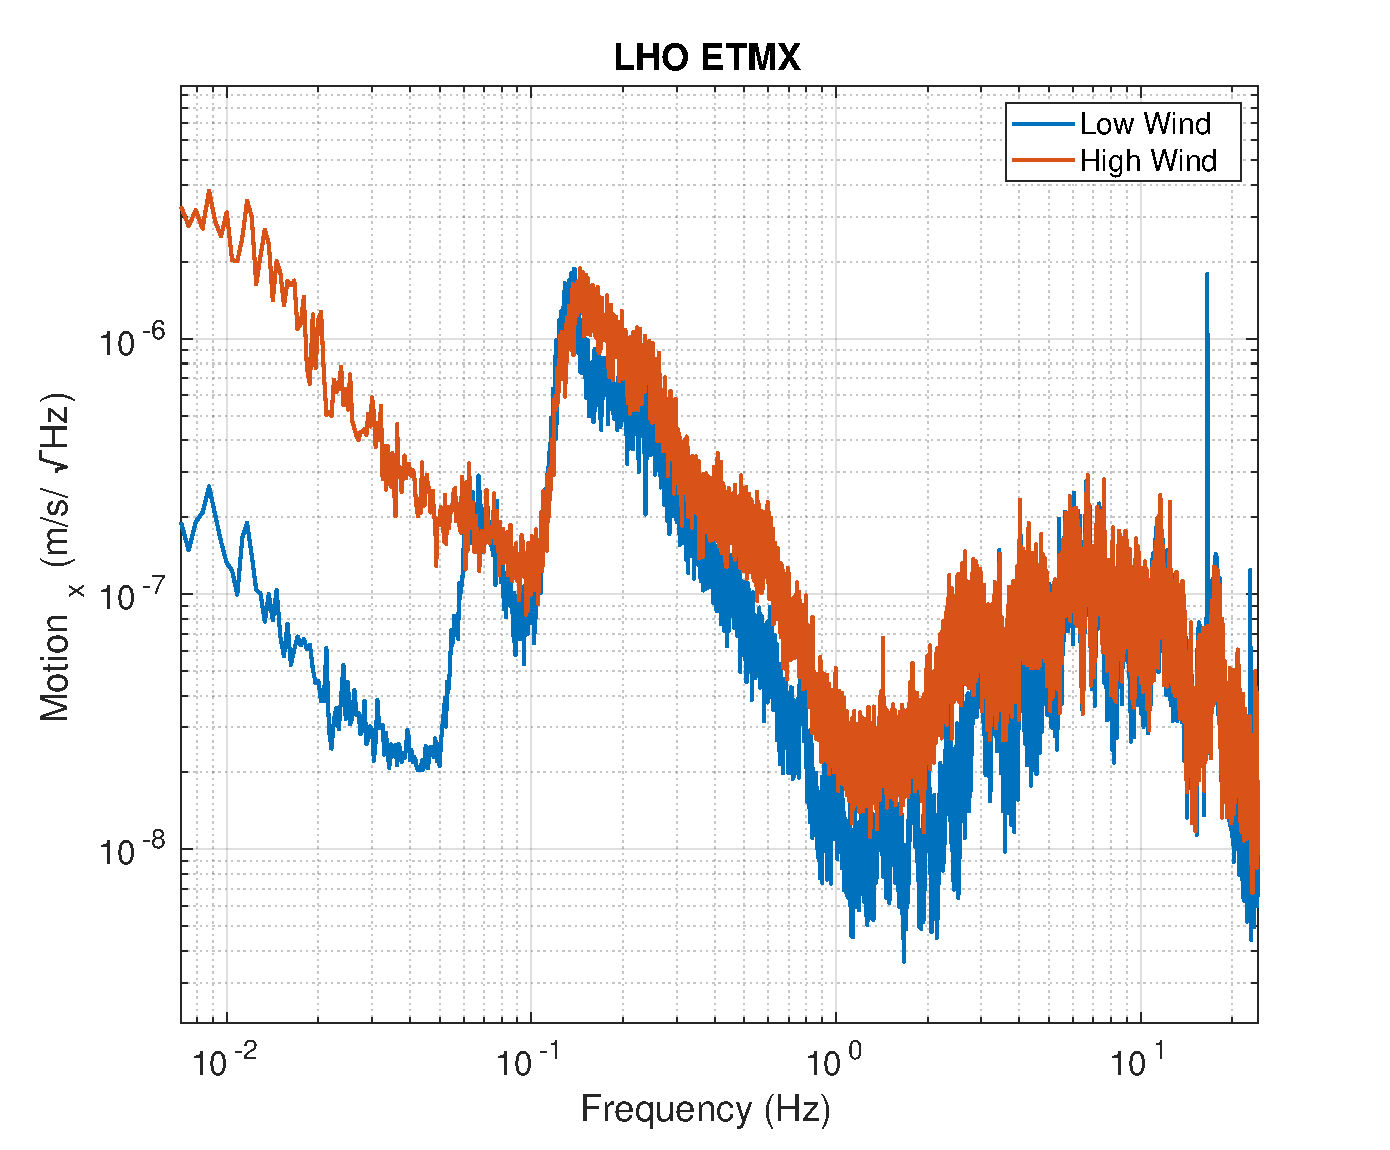
\includegraphics[width=0.75\textwidth]{windComp.pdf}
\caption{}
\label{wind}
\end{center}
\end{figure}

The dominate driver of ground tilts at the observatories is wind acting on the walls of the building. Although one would naiively assume that the wind would rigidly rotate the building, it was found that the true mechanism is differential pressure acting on the walls deforms the building's concrete slab. \textbf{cite?} 

\section{Sensor Correction with Tilt Subtraction}

\quad There are a few different ways to combat such a contamination. The most straight forward is to decrease the wind pressure by designing builds that don't interact with the wind as much or installing wind blocks such as wind fences or earth burms. Both of these option require significant construction and for the case of LIGO, tilt contamination was not known to be a problem when design the observatories. Another option is to build seismometers that are suspended in such a way that they do not experience tilts. This is an active area of research and may yield tilt-free seismometers. \textbf{cite}

The scheme that will be used here is to measure the tilt with an independent rotation sensor and subtract the wind driven contribution. This would then yield a channel of the following form:
\begin{align}
x_{seis}(\omega)=x_{trans}(\omega)+&\frac{g}{\omega^2}\theta_{wind}(\omega)\\
-&\frac{g}{\omega^2}\theta_{meas}(\omega)
\end{align}

where $\theta_{meas}$ is the tilt seen by the rotation sensor. Given a coherence $\gamma$ between the tilt component of the seismometer and rotation sensors this yields the following: \textbf{CHECK math}

\[x_{seis}(\omega)=x_{trans}(\omega)+\frac{g}{\omega^2}(1-\gamma)\theta_{wind}(\omega)\]

This is then a low tilt channel which can be used within the LIGO seismic isolation system.

\section{Mechanical System}

\quad The Beam Rotation Sensor (BRS) is a beam balance comprised of a 1-m long beam hung from two 10-15 $\mu$m thick beryllium-copper flexures. Figure \ref{BRS} shows a CAD model of the beam balance. 

\begin{figure}%
\begin{center}
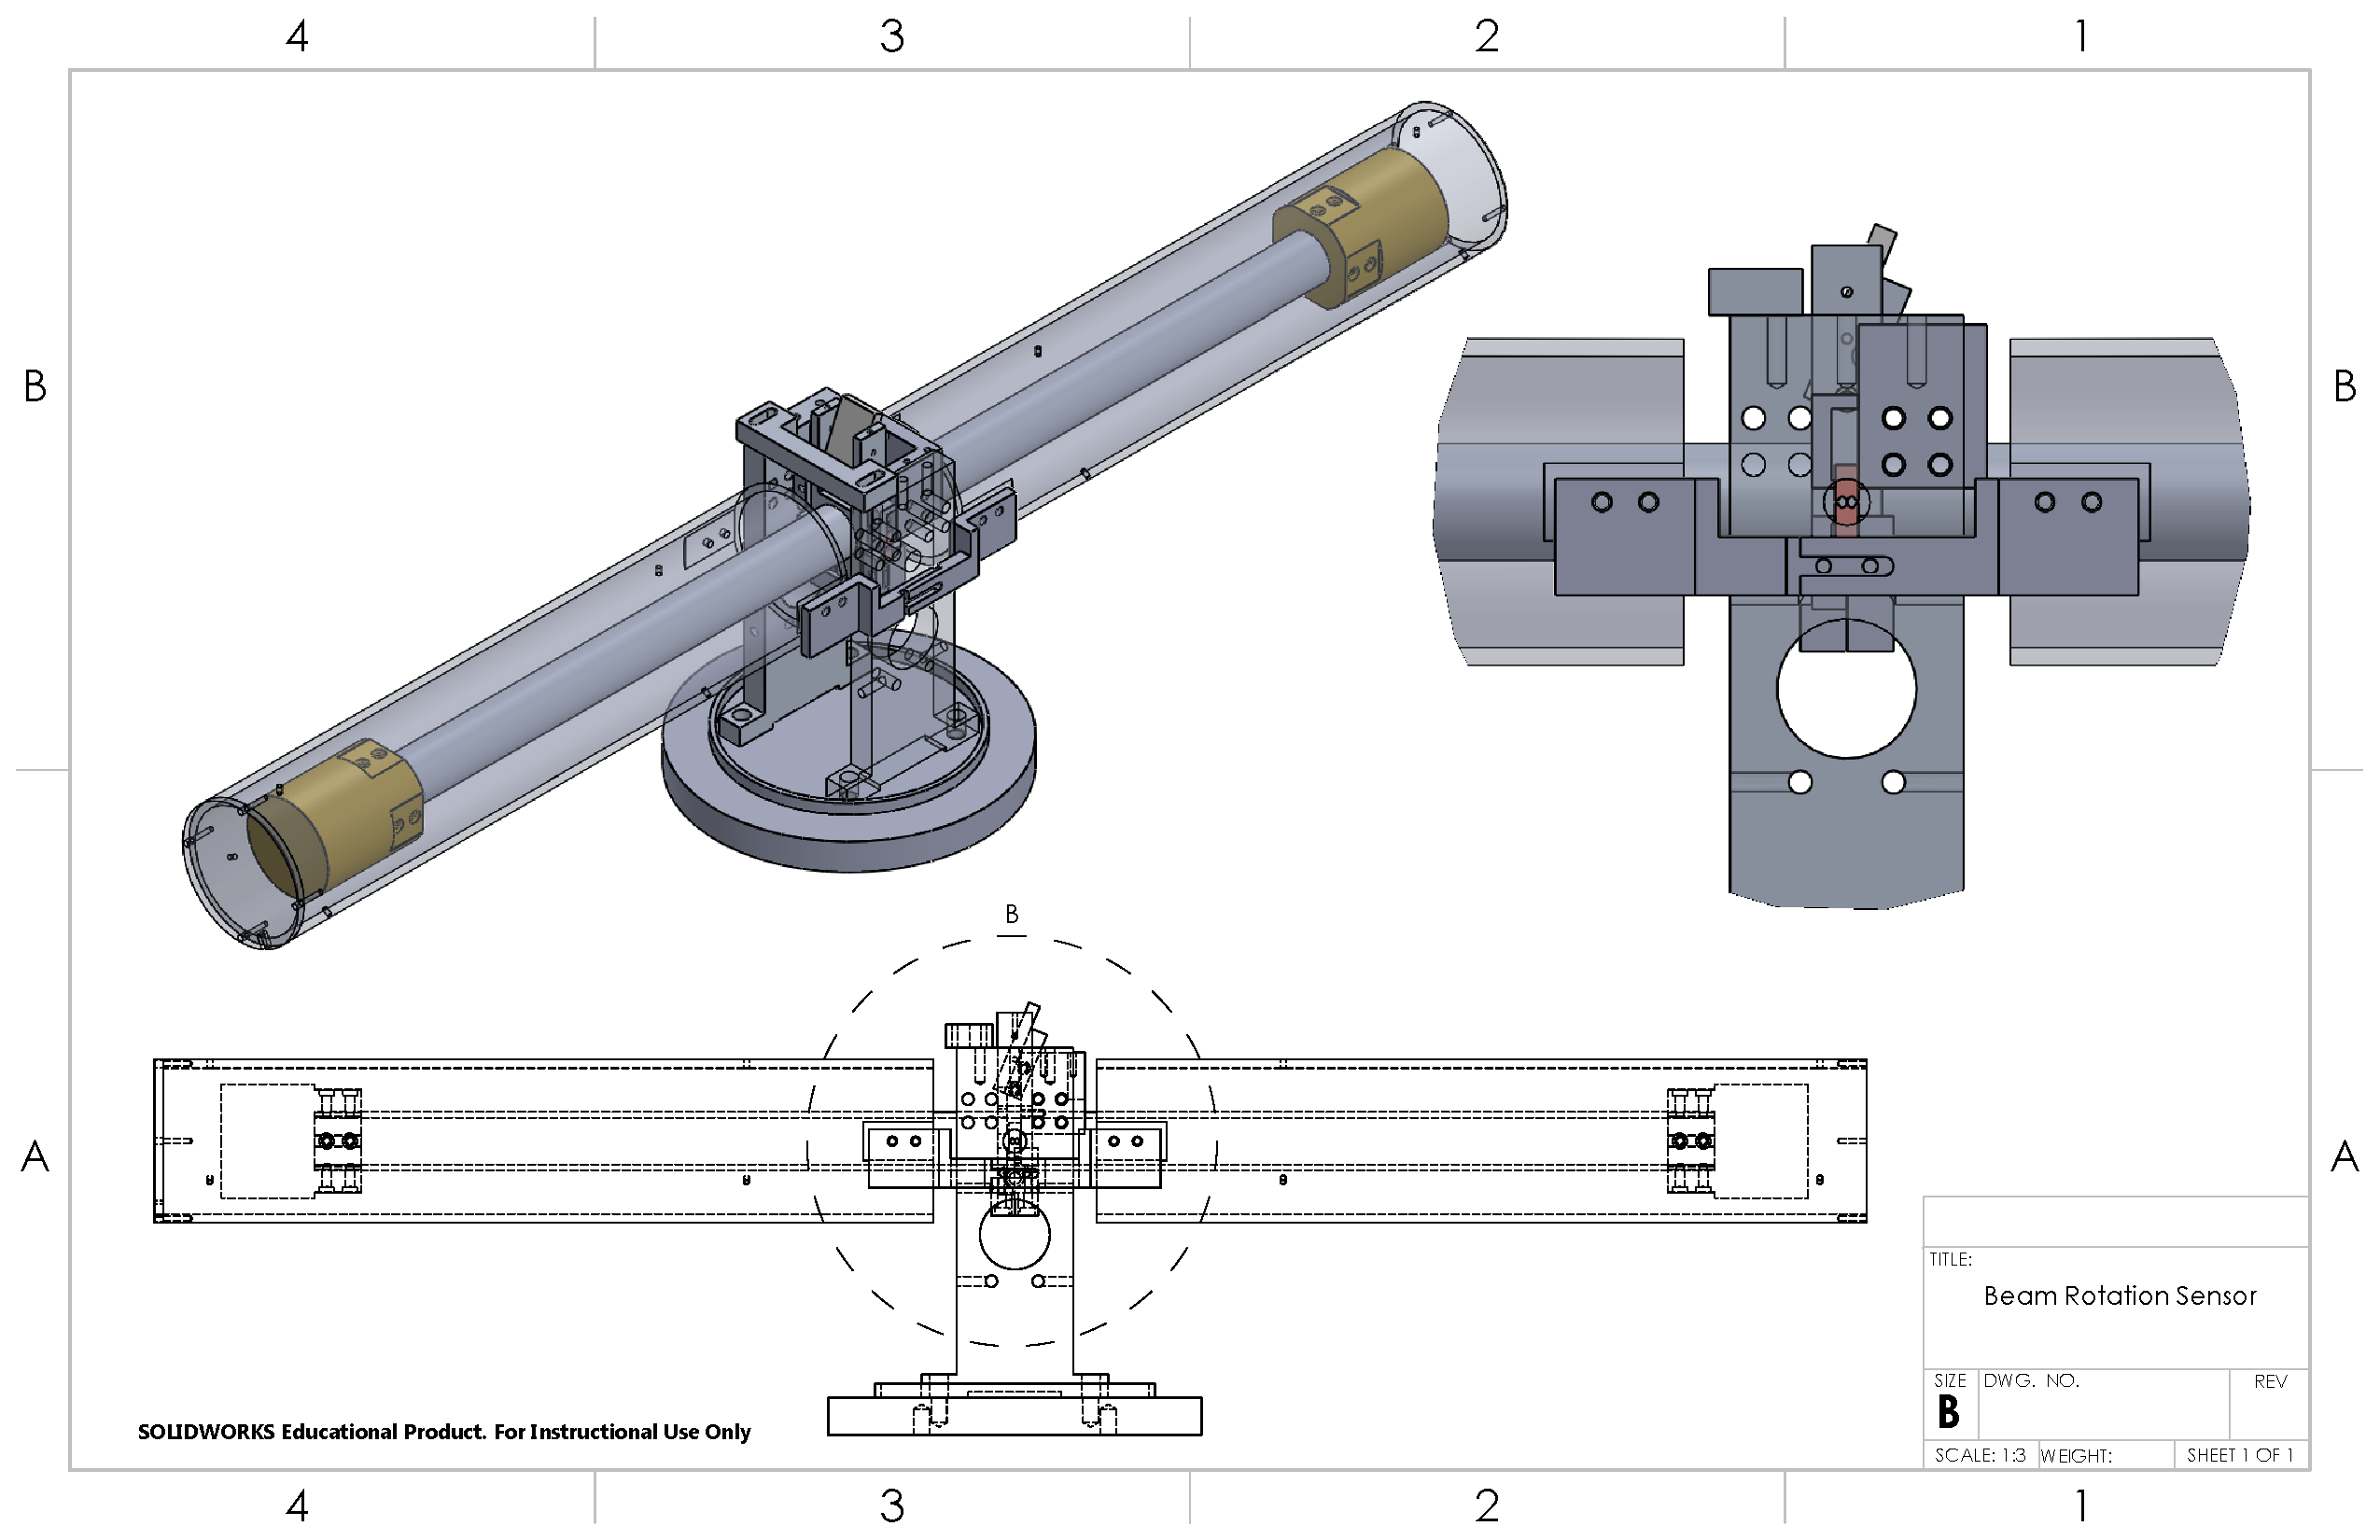
\includegraphics[width=\textwidth]{BRS_Drawing.PDF}
\caption{}
\label{BRS}
\end{center}
\end{figure}

This design makes the beam stiff in all degrees of freedom other than rotations around the horizontal axis which intersects the two flexure pivot points. This forms a system consisting of two elementary subsystems: a rotational spring mass system formed by the stiffness of the flexures, and a simple pendulum due to the offset of the pivot point and the center of mass. This is then described by the following equation of motion: \cite{venk2014}

\[I \ddot{\theta}(t)+\kappa (1+ \frac{i}{Q})(\theta(t)-\theta_p(t))+M g \delta \theta(t) +M \delta \ddot{x_p}(t)=\tau_{ex}(t)\]

where $\theta$ and $\theta_p$ are, respectively, the angle of beam and the platform with respect to gravitational vertical, $\tau_{ext}$ is the sum of all exterior torques, $I$ is the moment of inertia, $Q$ is the quality factor of the system, $\kappa$ is the spring constant of the flexures, $M$ is the mass of the balance, $g$ is the gravitational acceleration, $\delta$ is the vertical distance from the center of mass and the pivot point, and $x_p$ is the translation of the platform.

\textbf{derive translational coupling and readout equation}

In ideal operation, one would tune the center of mass to be at the pivot point and thus would produce a pure rotational spring-mass system with no translational coupling. In this limit, the rotation sensor is a rotational analog to a seismometer; above the resonant frequency as the casing rotates the beam stays inertial and thus allows one to measure the casing's rotation.

\section{Multi-Slit Autocollimator Readout}

\quad Optical levers are a simple optical angular readout which exploits the law of reflection to measure angular deflections of a mirror by observing the displacement of a reflected beam. The angle of the mirror is then described as:
\[\theta_{mirror}=\frac{x_{reflected}}{2d}\]
where $\theta_{mirror}$ is the angle of the mirror, $x_{reflected}$ is the displacement of the reflected beam, and $d$ is the distance between the optical system and the mirror. This allows one to increase the precious of the angular measurements arbitrarily by increasing $d$. However, with this comes a few disadvantages. One the effective gain of the sensor depends of the $d$ which may not be well known. Additionally, the system is sensitive to changes in $d$. 

An autocollimator adds a lens located one focal length from light source and the screen, shown in Figure \textbf{number}. This effectively replace the distance dependence with the focal length of the lens which allows the system to be only sensitive, to first order, to the angular motion of the mirror.

\textbf{autocollimator schematic}

To improve upon this further, a partially reflective mirror can be placed in between the optical system and the main mirror to act as a reference and allows for the subtraction of any motion of the optical system with respect to the main mirror. This yield a angular readout described by:
\[\theta_{mirror}=\frac{x_{main}-x_{reference}}{2f}\]

where $f$ is the focal length of the lens and $x_{reference}$ is the beam spot from the reference mirror.

\textbf{make table of BRS autocollimator parameters: focus, number of slits, slit width, CCD type, light source, frequency}

An increase in sensitivity can be made by employing a multi-slit autocollimator \cite{MSA}. This consists of an autocollimator with the light source replaced by a illuminated photomask of a number of thin slits. The pattern is then reflected off a set of reference and main mirror and imaged by a line CCD camera. These images are then analyzed to measure the distance between them thus yielding a measurement of angle. For the BRSs, this image analysis is achieved using bespoke software written in C\# which can be found at www.github.com/mpross/BRSReadout

To extract the distance between the patterns, the image goes through a series of steps to go from a vector of pixel intensities to a single angular output. When the software begins, the first frame that is captured is saved. All future frames are split into two, with one part representing the reference mirror and the other the main mirror. The cross correlation is then taken between each part and it's matching part from the first frame. This gives a curve who's maximum is located at the pixel number corresponding to separation between the pattern in the current frame and the first frame, which can be seen in Figure \textbf{number}. The points of this curve that are near the maximum are then fit to a Gaussian which allows for the extraction of the location of the peak with sub-pixel resolution. This is done for each pattern separately after which the difference between the reference pattern location and the main pattern location is taken. The difference is then proportional to the change in angle between the casing and the beam.

Compared to previous image analysis algorithms \cite{MSAPaper}, this algorithm is more computationally efficient while also being less susceptible to variations in the pattern image due to dust particulate, incorrect focusing, or beam clipping. A sensitivity of \textbf{$\sim$ 0.1 nrad$/\sqrt{\text{Hz}}$} was achieved with this autocollimator design and image analysis algorithm.

\section{Controls}

\quad As the BRSs are installed in active lab spaces, anthropogenic actively and environmental disturbances regularly apply torques on the beam balance, either through mechanical coupling through the flexures or gravitational coupling with the end masses. These can then cause the motion at the resonant frequency to rise to undesirable amplitudes. As the beam motion increases so does the noise. Additionally, some disturbances can be large enough to cause the amplitude to exceed the dynamic range of the autocollimator readout system.

The alleviate this issue, capacitor plates are installed underneath each end of the beam balance to act as actuators. The force between the two capacitor plates follows the following: 
\[F=\frac{\epsilon A V^2}{2d^2}\]
where $\epsilon$ is the permittivity of the material between the plates, $A$ is the area of the plate, $V$ is the voltage applied to the plates, and $d$ is the distance between the plates. The plate under the beam is connected to a DAC while the beam is grounded which allows for a controlled actuation torque to be applied to the beam. 

The control scheme that was adopted was one in which the feedback signal that is sent to the capacitors is the angular velocity of the beam band passed between 2 mHz and 20 mHz to include only motion at frequencies near the resonance. The feedback is additionally applied with low gain so that the feedback is only adding loss to the system as compared to locking the system in a strong feedback loop where all of the motion is absorbed into the control system. This is then implemented with two gain stages, a ``low amplitude'' stage which is always on and yields a Q of 10-15 and a ``high amplitude'' stage which is triggered if the amplitude rises above a threshold that is set based on the behavior of the given device and gives a Q of \textbf{number}.

\section{Noise Performance}
\section{Hanford Installation}

\quad Between the first (O1) and second (O2) observing runs of LIGO, two BRSs were installed at the LIGO Hanford Observatory, one at each end station correcting the translations along their respective arm. Although one would expect that the corner station sensors would also need to be corrected, a location was found within the corner station building which exhibited low tilt. \textbf{cite} This is thought to be due to the shape of the building the distance between this location and the walls. As such no BRS was necessary to achieve low tilt injection seismic isolation.

\begin{figure}%
\begin{center}
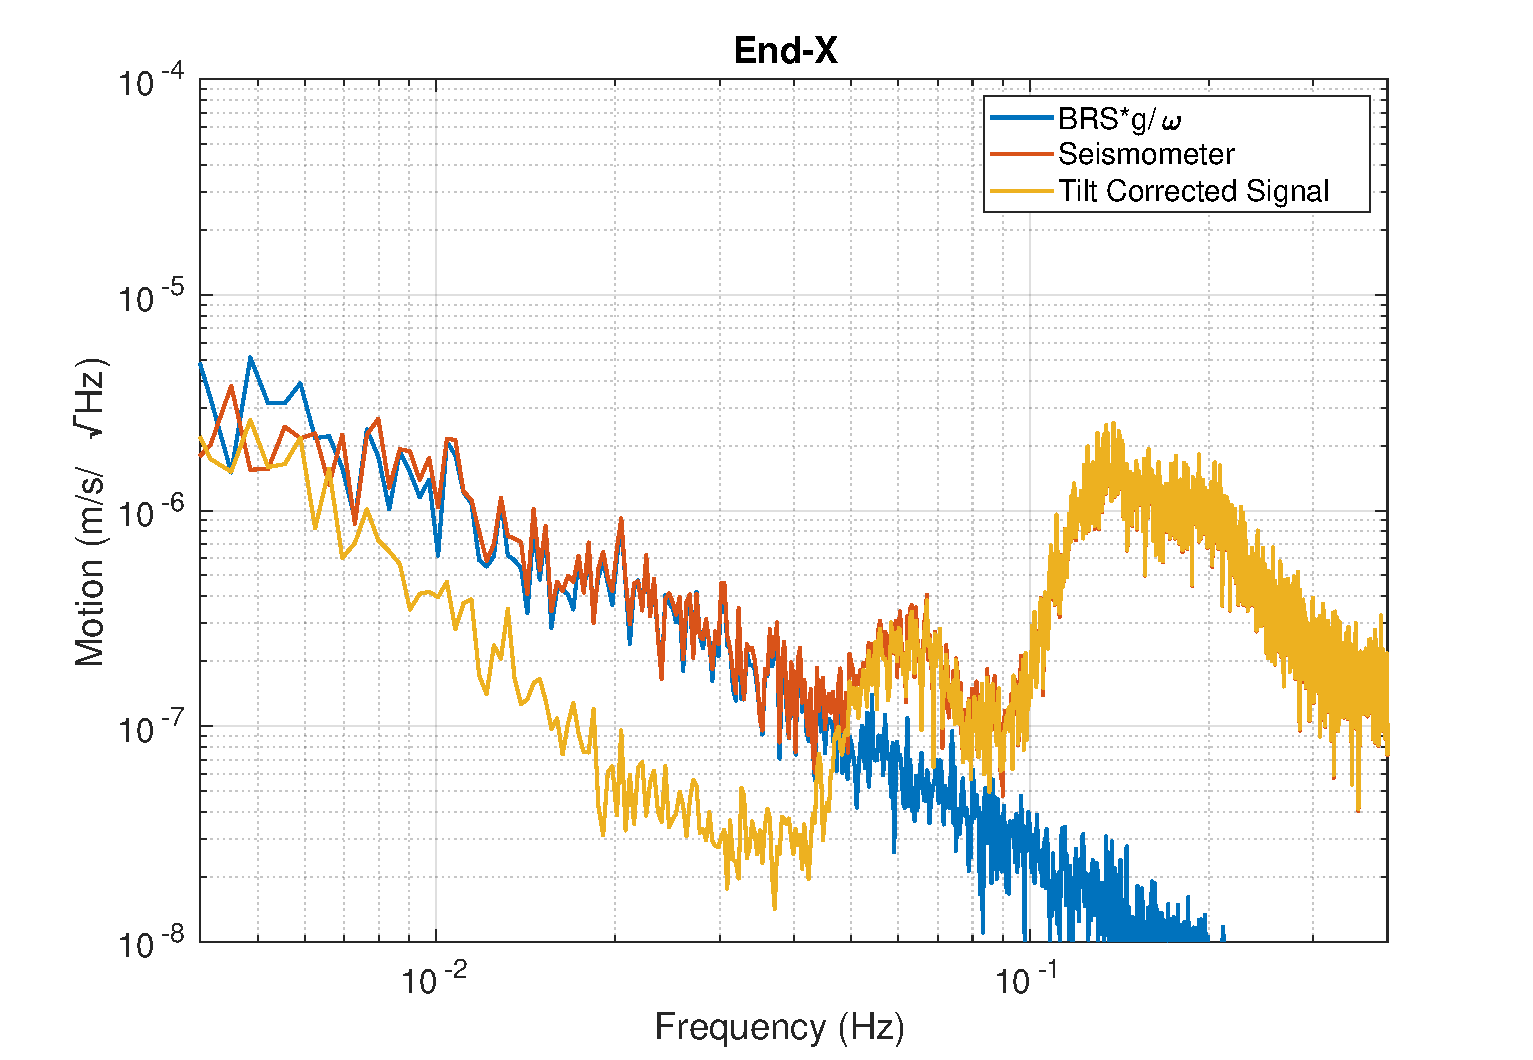
\includegraphics[width=0.75\textwidth]{HSubtractionETMX.pdf}
\caption{}
\label{sub}
\end{center}
\end{figure}

The tilt subtraction performance achieved with these devices can be seen in Figure \ref{sub} where it is evident that the system achieves tilt subtraction from around 6 mHz to 50 mHz. Above 50 mHz the seismometer signal is dominated by the oceanic microseism and the tilt contribution is negligible. Below 6 mHz, the BRS signal becomes overwhelmed by instrumental noise. This performance can also be seen in Figure \ref{subTime} which shows a example time series of the tilt subtraction. 

\begin{figure}%
\begin{center}
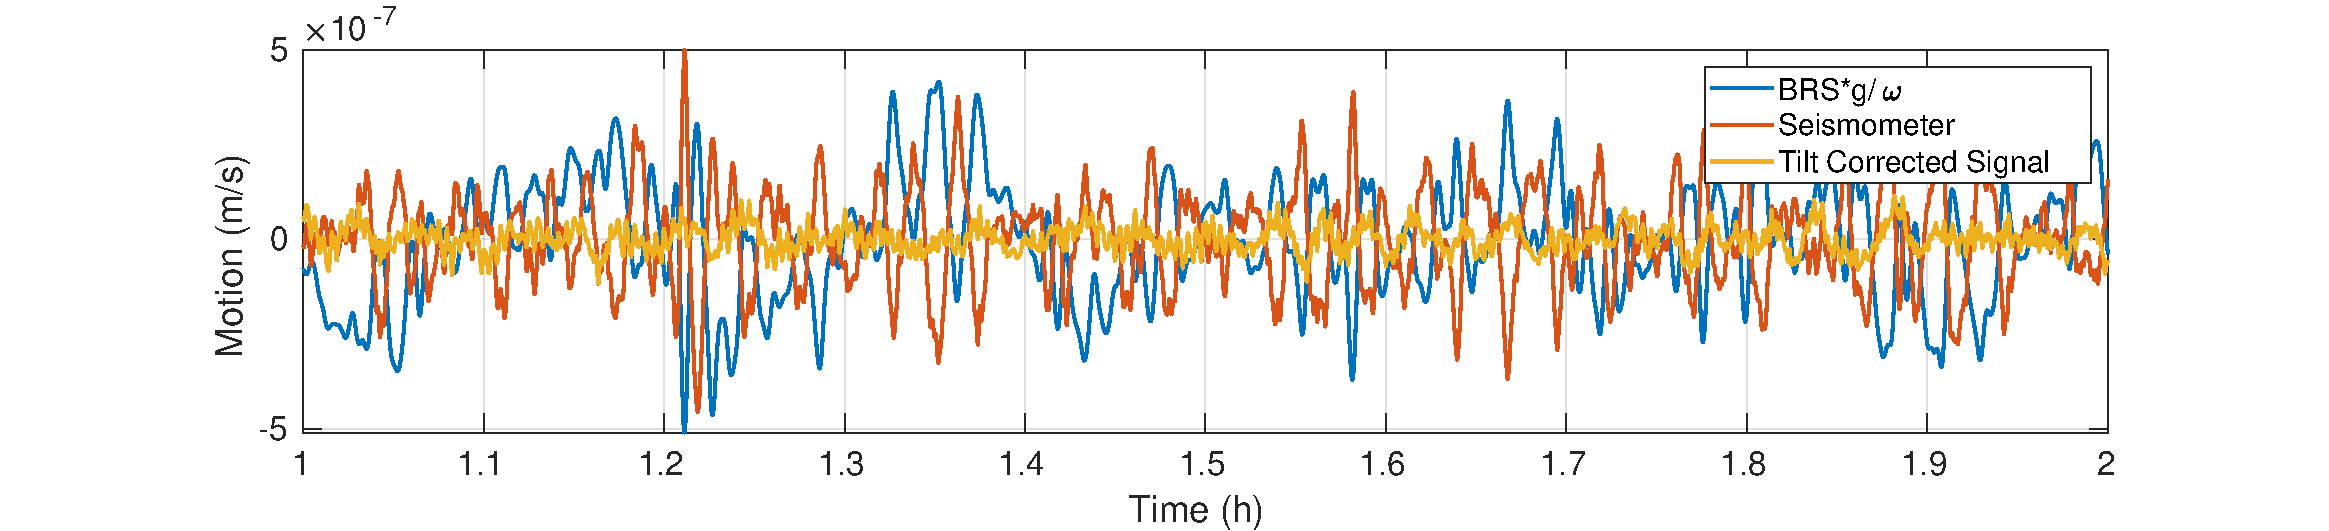
\includegraphics[width=\textwidth]{TiltCorrTime.pdf}
\caption{}
\label{subTime}
\end{center}
\end{figure}

This tilt subtracted channel was then used as the ground signal for the isolation's sensor correction instead of the raw seismometer. Along with the use of the low tilt seismometer for the corner station, the addition of the BRSs in the seismic control scheme yielded significant improvements in the ability to lock the interferometer at increased wind speeds which can be seen in Figure \ref{O2}

\begin{figure}%
\begin{center}
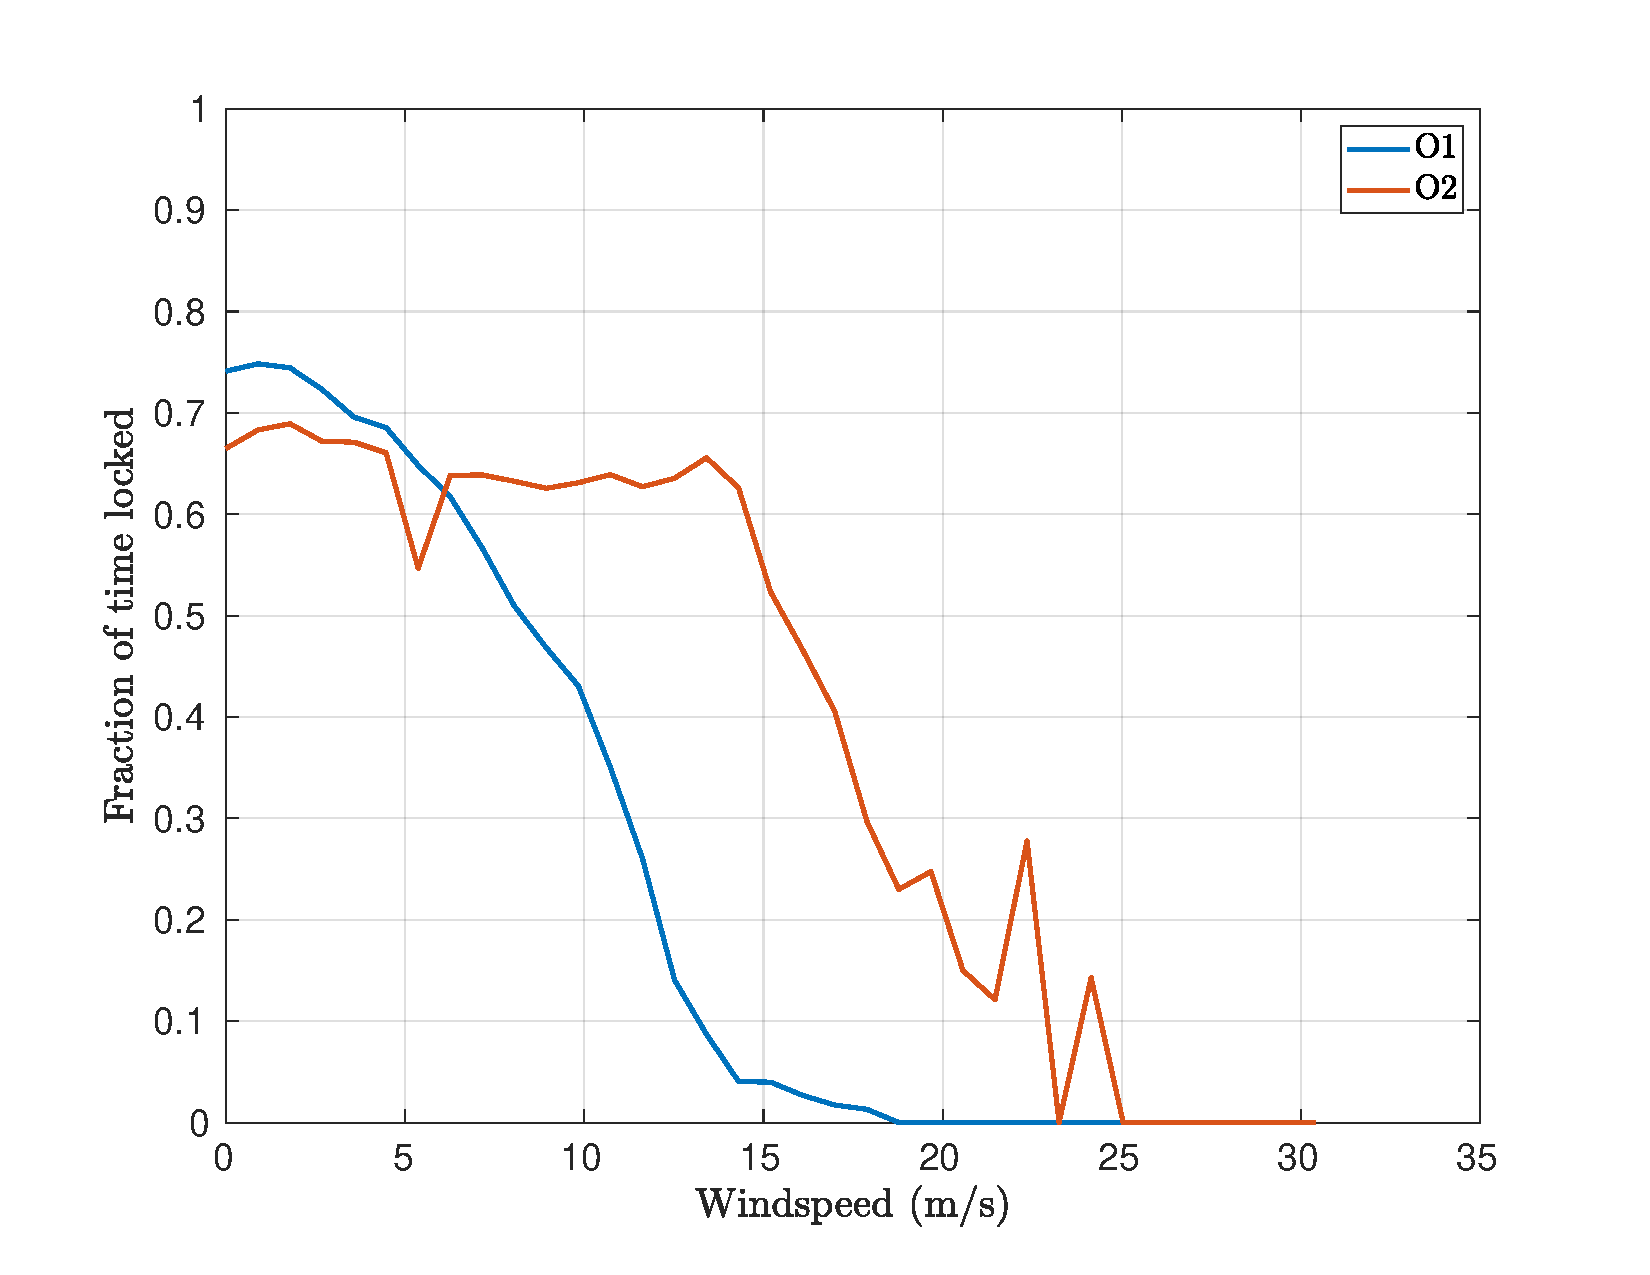
\includegraphics[width=0.75\textwidth]{Wind_LockedFraction_total.pdf}
\caption{}
\label{O2}
\end{center}
\end{figure}

\section{Livingston Installation}

\quad After the success of the Hanford BRS installation, four devices were installed at the LIGO Livingston Observatory (LLO) between the second and third (O3) observing runs. Due to differences in the size and shape of the corner station building at LLO a low tilt location was not found. Thus two BRSs were installed located near the two input test masses (ITM) correcting the seismometer signal oriented along their respective arms. 

All four were implemented in a similar fashion as the Hanford devices.

\chapter{30-cm Scale On-Board Rotation Sensors}
\section{Angular Controls}
\section{Mechanical System}
\section{Interferometric Readout}
\section{Controls}
\section{Noise Performance}

\chapter{Applications}
\quad The development of these highly sensitive rotation sensors have opened up a few novel scientific avenues that have been explored and many that have not.

\section{Geophysics}
Seismic waves have six components, three translations and three rotations, however seismology has long neglected the rotational components due the lack of sensitive rotation sensors. Recent developments have begun to alleviated this issue with the advent of seismically relevant ring laser gyros. \textbf{cite Gryo} The BRSs described above join a small class of ground rotation sensors with high enough sensitivity at low frequency to allow for the use in seismology.
\subsection{Rayleigh Wave Theory}
\subsection{Wave Field Parameter Extraction}
\subsection{Single Station Dispersion Measurements}
\section{Newtonian Noise}
\subsection{Theory}
\subsection{Observations}

\bibliographystyle{apalike}
\bibliography{Dissertation}
\printendnotes
\nocite{*}   
\bibliographystyle{plain}
\bibliography{Dissertation}
\end{document}


